
\chapter{The transmission of the Welsh laws}
\label{cha:welsh-laws}

% \section{Some quotes, tables, and stemmas}
% \label{sec:some-quotes-tables}


% \begin{figure}[h]
  \centering
  \begin{tikzpicture}[font=\itshape,level distance=10mm]
    \node(A){A}
    child {node {E}
      child [missing]
      child [missing]
      child {node(B) {B}}
    }
    child [missing]
    child {node(C) {C}}
    ;
    \draw(B)--(C)
    ;
    \node[right= 1em of C](S){\upshape saec.~XIII\textsuperscript{med}};
    \node[right= 5em of A]{c.~\upshape 1200};
    \node[right= 5em of B]{c.~\upshape 1282};
  \end{tikzpicture}
  \caption{Gwenogvryn Evans's \mw{Llyfr Iorwerth}, from \textcite{charles-edwards_textual_2016}.}
  \label{fig:gwevanslli}
\end{figure}

\begin{figure}[h]
  \centering
  \begin{tikzpicture}[font=\itshape]
    \node{X}
    child {node(alph) {α}
      child {node(B) {B}}
    }
    child {node (beta) {β}
      child {node(C) {C}}
      child {node (gamma) {γ}
        child {node (delta) {δ}
          child{node{A}}
          child{node{E}}
        }
        child[missing]
        child {node (eps){ε}
          child {node{D}}
          child{node{ζ}
            child {node {Col}}
            child {node {\upshape Llanforda}}
          }
        }
      }
    }
    ;
    \node[left=of alph](nalph){Galanas B \upshape added};
    \node[left= of B](nB){{\upshape no} damweiniau};
    \node[below left= of C](nC){{\upshape no} damweiniau};
    \node[below left=of delta,align=left](ndelta){- {\upshape Pref.\ to Test Bk.}\\+ Br.\ Gwŷr Arfon};
    \node[right=of beta](nbeta){+ Galanas E \upshape\& Pref.\ to Test Book};
    \node[right=of gamma](ngamma){+ Damweiniau I};
    \node[right=of eps](neps){+ Damweiniau II};
    \draw[dotted](alph)--(nalph);
    \draw[dotted](B)--(nB);
    \draw[dotted](C)--(nC);
    \draw[dotted](delta)--(ndelta);
    \draw[dotted](beta)--(nbeta);
    \draw[dotted](gamma)--(ngamma);
    \draw[dotted](eps)--(neps);
  \end{tikzpicture}
  \caption{Wiliam's \mw{Llyfr Iorwerth}, simplified by \textcite{charles-edwards_textual_2016}.}
  \label{fig:wiliamiorwerth}
\end{figure}

%  \begin{figure}[h]
%     \centering
% \begin{tikzpicture}[font=\itshape]
% \node{\upshape Redaction I} 
% child {node {α}
%   child [level distance=15mm]{node {A}}
%   child [level distance=15mm]{node {E}}
% }
% child [xshift=1em]{node {\upshape Redaction II}
%   child [grow=down] {node {β}
%     child [level distance =10mm,xshift=-1em]{node {C}}
%     }
%     child[level distance=20mm] {node{γ}
%       child [level distance=15mm]{node {\vphantom{J}GDLew}}
%       child [level distance=15mm]{node{BJKTim}}
%     }
% }
%     ;
%   \end{tikzpicture}
%     \caption{A stemma of the Laws of the Country  according to Thomas Charles-Edwards.}
%     \label{fig:stemmalawc}
%   \end{figure}
  
  \begin{figure}[h]
    \centering
    \begin{tikzpicture}[font=\itshape,level distance=17.5mm]
\node(1){\upshape Redaction I} 
child {node {α}
  child{node(A) {A}}
  child{node(E) {E}}
}
child[missing]
child {node(2) {\upshape Redaction II}
  child {node[align=center] (beta){β}
    child [dashed,level distance=35mm]{node(B) {\vphantom{J}B}
      edge from parent node [midway,above,sloped]{Test Book}}
    child {node {C}}
    child[missing]
  }
  child[missing]
  child {node(gamma){γ}
    child  {node {GDLew}}
    child[missing]
      child [level distance=35mm]{node {JKTim}
      edge from parent node (J){}  
      }
  }
}
  ;
  \node[above left=of E](nA){Bees I \& II};
  \node[below left=of beta,xshift=-15mm](nbeta){Bees I};
  \node[right=of 1](n1){Bees I \& II};
  \node[right=of 2,align=center](n2){+ Preface to Test Book\\ Bees I \& II};
  \node[right=of gamma,align=center](ngamma){+ Hywel to Rome\\Bees II};
  \draw[dotted](A)--(nA) -- (E);
  \draw[dotted](beta)--(nbeta);
  \draw[dotted](1)--(n1);
  \draw[dotted](2)--(n2);
  \draw[dotted](gamma)--(ngamma);
  \draw[dashed](B) to  node [midway,below,sloped]{Laws of Country}  (J);
\end{tikzpicture}
\caption{A stemma of \mw{Llyfr Iorwerth} manuscripts according to \textcite{charles-edwards_textual_2016}. Dashed lines indicate partial transmission.}
\label{fig:stemmatestb}
\end{figure}

\begin{figure}[h]
  \centering
  \begin{tikzpicture}[font=\itshape]
    \node{X}
    child{node{α}
      child{node{γ}
        child{node{A}}
        child{node{E}}
      }
      child{node{C}}
    }
    child[missing]
    child{node{β}
      child{node{δ}
        child{node{D}}
        child{node{Lew}}
      }
      child[missing]
      child{node{ε}
        child{node{G}}
        child{node{ζ}
          child{node{J}}
          child{node{B}}
          child{node{K}}
          child{node{Tim}}
        }
      }
    }
  ;
  \end{tikzpicture}
  \caption{Stemma of Ior's tractate on suretyship \autocite[138]{charles-edwards_lawyers_1986}}
  \label{fig:suretyshstemma}
\end{figure}



\begin{spacing}{1}
  \itshape
  \begin{pages}
    \begin{Leftside}
      \beginnumbering
      \pstart[
      \subsection*{C 180ra1--180va23}
      \label{sec:parallel-text-c-1}
      ]
      \textup{/180ra/} Hewel \al{ỽ}ap kadell \al{t}ewyssaỽc kemry a deỽynnỽs attaỽ chwe gwyr o \al{p}ob kantref eg kemry oll hyt e ty gwyn en dyỽet a henny or gwyr doethaf en e \al{k}eỽoeth. e pedwar onadỽnt en llegyon ar deỽ en escolheygyon. Sef achaỽs e dwcpwyt er escolheygyon rac dody or lleegyon petheỽ a \al{ỽ}ey en erbyn er escrethỽr \al{g}lan. Ac esef amser e doethant eno petheỽnos amys \al{g}arawys. ac esef achaỽs e doethant eno e \al{g}arawys ỽrth na dely nep na dewedwyt kam nay \al{g}wneỽthỽr en er amser gleyndyt hỽnnỽ.
      \pend
      \pstart
      Ac ena ed edrychassant e kyỽreythyeỽ. ar hon a \al{ỽ}ey re \al{t}rom onadỽnt y hescaỽynhaỽ. ar hon a \al{ỽ}ey re eskaỽyn onadỽnt yhachwanegỽ. Peth or kyỽreythyeỽ a \al{a}dassant \al{ỽ}al ed oeydynt. peth arall a \al{ỽ}ynnassant y emendaỽ. ereyll a dyleassant \textup{/180rb/} en \al{k}ỽbyl. ac ereyll o newyd a \al{o}ssodassant.
      \pend
      \pstart
      Ac ena e dodassant hewel a henny o doethyon eỽ hemendyth ar nep a \al{k}amarỽerey or kyỽreythyeỽ henny ac ar er arglwyd ay semỽtey yr ỽn onadỽnt namyn kan dỽỽndep kynnỽlleytỽa \al{k}ymeynt ac a \al{w}u eno. ER eyl emendyth a dodassant ar er arglwyd ay rodey. ac ar e dyn ay kymerey \al{t}eylygdaỽt egneydyaeth ar ny \al{g}wyney teyr koloỽyn kyỽreyth a gwerth gwyllt a dof. ac a \al{p}erthyn attadỽnt
      \pend
      \pstart
      \pend
      \pstart
      Pwy \al{b}ynnac a \al{ỽ}ynho kymryt egneydyaeth \al{ỽ}al hy e mae yaỽn ydaỽ gwybot e llyỽyr hỽn. \al{ỽ}al e bo teylỽng. ydaỽ kymryt egneydyaeth. a phan \al{g}welo y athro y \al{ỽ}ot yn \al{t}eylỽng. ellyget ar er egnat llys ef. ar egnat llys \al{p}yeỽ y \al{p}roỽy. Ac os gwyl en \al{t}eylỽng enteỽ \al{p}yeỽ y ellỽng ef ar er arglwyd. ar arglwyd \al{p}yeỽ estynnỽ ydaỽ enteỽ egneydyaeth. ac en \al{ỽ}arnedyc e \al{ỽ}raỽt a \al{ỽ}arnho enteỽ o henny allan. Ac enteỽ \al{p}yeỽ rody pedeyr ar ỽgeynt yr egnat llys en y \al{o}byr. O derỽyd ydaỽ enteỽ barnỽ kam \al{ỽ}raỽt o henny allan ny dely enteỽ y \al{t}aỽaỽt \textup{/180va/} onys pryn yr y \al{w}erth kyỽreyth. O derỽyd emwystlaỽ ac enteỽ. ae \al{ỽ}ot enteỽ ar er yaỽn. ef adely wynepwarth y \al{g}an e nep a emwystlo ac ef. a chamlỽrỽ yr arglwyd. Ny dely egnat kymryt gwystyl onys myn ehỽn gwedy del oe \al{ỽ}raỽtle. ac ny dely kymryt y \al{g}an \al{l}eyc onyt kan adaỽ braỽt a \al{ỽ}o gwell y \al{g}an egnat arall nor hon a \al{ỽ}arnỽs ef.
      \pend
      \pstart
      Ar lleỽyr hỽn a \al{g}ynỽllỽs yorwerth \al{ỽ}ap madaỽc o \al{l}yỽyr kyỽnerth \al{ỽ}ap morgeneỽ. ac o \al{l}yỽyr gweyr \al{ỽ}ap rỽuaỽn. ac o \al{l}yỽyr Goronwy \al{ỽ}ap morydyc. ac y \al{g}yt a hennyor llyỽreỽ goreỽ a kaỽas heỽyt eg gwyned. a phowys. a deheỽparth. ar llyỽyr hỽn a \al{e}lwyr e llyỽyr praỽ. Sef ew henny teyr koloỽyn \al{k}yỽreyth. a gwerth gwyllt a dof. ac a \al{p}erthyn ar henny.
      \pend
      \endnumbering
    \end{Leftside}
    \begin{Rightside}
      \beginnumbering
      \pstart[
      \subsection*{D 55v20--57r2}
      \label{sec:d}
      ]
      \textup{/55v/} Howel \al{v}ab kadeỻ \al{t}ywyssaỽc kymry a dyuynnaỽd attaỽ chwe gwyr o \al{b}op kantref yng kymry hyt y ty gwynn yn dyuet. a hynny or gỽyr doethaf yn y \al{g}yuoeth. y pedwar onadunt yn ỻeygyon. ar deu yn yscolheigyon. \textup{/56r/} rac dodi or ỻeygyon petheu a \al{v}ei yn erbyn yr ysgruthyr \al{l}an. Sef amser y doethant yno; pythewnos a mis \al{g}arawys. ỽrth na dylyei neb na dywedut cam nae \al{w}neuthur yn yr amser gleindyt hỽnnỽ.
      \pend
      \pstart
      Ac yna yd edrychassant y kyfreitheu; yr honn a \al{v}ei ry \al{d}rom y chosp onadunt. y ỻeihau. ar honn a \al{v}ei ry \al{v}echan; y hachwanegu. Peth or kyfreitheu a \al{a}dassant \al{u}al yd yttoedynt peth araỻ a emendanassant. ereiỻ o \al{g}ỽbyl a dileassant.
      \pend
      \pstart
      ac yna y dodassant eu hemeỻtith howel a hynny o doethon ar yr arglỽyd a symuttei vn or kyfreitheu hynny; namyn \al{g}an duundeb kynnuỻeitua \al{g}ymeint a honno. ar eil emeỻtith a dodassant ar yr arglỽyd ae rodei. ac ar y dyn a \al{g}ymerei arnaỽ \al{d}eilygdaỽt ygneityaeth ar ny \al{w}ypei \al{t}eir kolofyn kyfreith. a gỽerth gỽyỻt a dof. ac a \al{b}erthyn attunt.
      \pend
      \pstart
      A gỽedy gỽneuthur ohonunt y kyfreitheu \al{u}al y tebygynt eu bot yn \al{d}eilỽg; yd aeth howel ac escob mynyỽ. ac escob assaf. ac escob bangor. ac y am hynny yny \al{v}u ar y \al{d}rydyd ar dec o athraỽon a doethon ereiỻ o \al{l}eygyon. ac yd aethant hyt yn ruuein. y \al{g}ymryt aỽdurdaỽt pab ruuein y \al{g}yfreitheu howel. ac yna y darỻewyt kyfreitheu howel rac bronn \al{p}ab ruuein. ac y bu \al{u}odlaỽn y pab udunt. ac y rodes y aỽdurdaỽt udunt. \textup{/56v/} ac y doeth howel ae \al{g}edymdeithon adref. Ac yr hynny hediỽ yd ydys yn daly o \al{g}yfreitheu hoỽel.
      \pend
      \pstart
      Pỽy \al{b}ynnac a \al{v}ynno kymryt ygneityaeth arnaỽ; \al{v}al hynn y mae idaỽ gỽybot y ỻyfyr hỽnn. \al{u}al y bo teilỽg idaỽ kymryt ygneityaeth. a phan \al{w}elo y athro y \al{v}ot yn \al{d}eilỽg; goỻyget ef att yr ygnat ỻys. ar ygnat ỻys \al{b}ieu y \al{b}roui. ac os gỽyl yn \al{d}eilỽg; ynteu \al{b}ieu y oỻỽg ef att yr arglỽyd. ar arglỽyd \al{b}ieu estynnu ygneityaeth idaỽ. ac yn \al{u}arnedic y \al{v}arn a \al{v}arnho o hynny aỻan. ac ynteu \al{b}ieu rodi pedeir ar hugeint yr ygnat ỻys yn y \al{o}byr. O deruyd idaỽ ynteu \al{v}arnu camvraỽt o hynny aỻan; ny dyly y \al{d}auaỽt ony s pryn yr y \al{w}erth kyfreith. O deruyd. ymwystlaỽ ac ynteu ae \al{v}ot ef ar yr iaỽn; ef a dyly wynebwerth y \al{g}an y neb a ymỽystlo ac ef. a chamlỽrỽ yr arglỽyd. Ny dyly ygnat kymryt gỽystyl gỽedy del oe \al{v}raỽtle. ony s mynn. ac ny dyly y \al{g}ymryt y \al{g}an \al{l}eyc; onyt \al{g}an adaỽ braỽt a \al{v}o gỽeỻ y \al{g}an araỻ nor \al{v}raỽt a \al{v}arnaỽd ef.
      \pend
      \pstart
      Y ỻyfyr hỽnn a \al{g}ynnuỻaỽd Jorwerth \al{u}ab madaỽc. o \al{l}yfyr kyfreith Morgeneu. a ỻyfyr gỽeir \al{u}ab ruaỽn. a ỻyfyr gronỽy \al{u}ab Moridic. ac y\al{g}yt a hynny or ỻyfreu goreu yg gỽyned. a phowys. a deheubarth. ar ỻyfyr hỽnn a \al{e}lwir ỻyfyr praỽf. Sef \textup{/57r/} yỽ hynny; teir kolofyn \al{k}yfreith. a gỽerth gỽyỻt a dof. ac a \al{b}erthyn ar hynny.
      \pend
      \endnumbering
    \end{Rightside}
  \end{pages} 
  \Pages
\end{spacing}

%%% Local Variables:
%%% mode: latex
%%% TeX-master: "../main"
%%% End:



% \section{Research plan for the laws}
% \label{sec:research-plan-laws}

\section{Introduction}
\label{sec:introduction}

In this chapter, I analyze where \lT\ was represented in the various law texts.
This allows me to see under what circumstances scribes copying manuscripts maintained or changed the non-representation of \lT.

I expect that most instances of \lT\ were represented by the mid-fourteenth century, so manuscripts from around this period are most useful to chart the change in orthography.
Earlier manuscripts serve to demonstrate that the law texts indeed saw a period in which lenition of voiceless stops was not represented, even though lenition of other consonants was.
 Later manuscripts may still show traces of the early orthography, allowing me to identify specific environments within which non-representation of lenited voiceless stops may be preserved.
 I focus on the transmission of \mw{Llyfr Iorwerth}, because most of the oldest law manuscripts contain this law text, while there are still some newer ones.

% How are various manuscripts related to each other?
% It is nowadays thought that none of the earliest extant manuscripts is a direct ancestor of another extant copy.
% One author who did think this was J.\ Gwenogvryn Evans (Figure~\ref{fig:gwevanslli}).
% Rather, extant manuscripts are held to have common exemplars that no longer exist.
% Figure~\ref{fig:stemmatestb} gives a stemma for the Iorwerth manuscripts (and some more manuscripts), and I will use this stemma as a point of departure for my own research.

% Which manuscripts may be used for analysis?
% One useful manuscript is \textit{A}, the \gls{bbch}, dating from around 1250. This manuscript is one of the oldest law manuscripts, and its orthography is very unusual.
% Another useful manuscript is \textit{B}, which is also fairly old, and dates from the end of the thirteenth century.
% Other thirteenth-century manuscripts shown in Figure~\ref{fig:stemmatestb}: \textit{EC};
% early fourteenth century: \textit{G};
% other manuscripts in this stemma are all later than the fourteenth century.
% Some more useful manuscripts are: \textit{VW}, by scribe X86; \textit{Tr}, by Gwilym Was Da.

% What sections of the law texts are useful for analysis?
% Figure~\ref{fig:stemmatestb} shows that \textit{B} was  transmitted in part from several sources. This makes both the Test Book and the Laws of Country interesting targets for analysis, as the orthography of lenition may confirm or deny this peculiar reconstruction by Charles-Edwards.
% Figure~\ref{fig:stemmatestb} also shows that different parts of the Test Book may have been added in intermediate stages between Redaction I and the extant manuscripts.
% Comparison of these chunks with text found in all the manuscripts may prove useful in establishing at what point in time these chunks were added, and therefore when some of the hypothetical nodes in the stemma were written.

% \subsection{The law corpus}
% \label{sec:fleshed-out-research}
I will take a part of the tractate on suretyship for analysis.
This tractate is found in many manuscripts from the Iorwerth tradition, and those manuscripts vary in date from the mid-thirteenth century to 1404.
To be more specific, I will use \textcite[\S\S58--65]{wiliam_llyfr_1960} for analysis. These paragraphs correspond to the folio numbers, column numbers and line numbers in the manuscripts given in Table~\ref{tab:surety}. This text runs continuously in all of these manuscripts, except in \gls{sG}, where it is interspersed with other additions. Over 200 data points were taken from each manuscript for analysis.
\begin{table}[h]
  \centering
  \begin{tabular}{@{}lddld@{}}
    \toprule
    MS                       & Begin                                     & End     & Date                                        & Data pts          \\ \midrule
    \gls{sA}                       & 43.22                                     & 48.11   & s.xiii\textsuperscript{med}                                  & 210                  \\
    \gls{sB}                       & 20r.22                                    & 23v.17  & s.xiii\textsuperscript{2}                 & 234                  \\
    \gls{sC}                       & 155va.10                                  & 161ra.7 & s.xiii\textsuperscript{med}                                  & 229                  \\
    \gls{sD}                       & 52.19                                     & 61.16   & ca.\ 1404                      & 231                  \\
    \gls{sE}                       & 34.5                                      & 39.13   & s.xiii\textsuperscript{2}                 & 218                  \\
    \multirow{2}{*}{\gls{sG}}      & 20r.1                                     & 23v.6   & \multirow{2}{*}{s.xiv\textsuperscript{1}} & \multirow{2}{*}{263} \\
                             & 26r.1                                     & 26v.12  &                                             &                      \\
    \gls{sK}&68.19 & 77.23 & s.xv\textsuperscript{2}& 244 \\
    \bottomrule
  \end{tabular}
  \caption{The parts of each manuscript containing the relevant paragraphs of the tractate on suretyship in various recensions of \mw{Llyfr Iorwerth}.}
  \label{tab:surety}
\end{table}

\section{On the manuscripts}
\label{sec:manuscripts}
Here, I discuss the date and place where the manuscripts used are thought to be written.

\section{On the stemmata}
\label{sec:stemmata}
Here, I discuss the literature on how the manuscripts are related.


\begin{figure}[h]
  \centering
  \begin{tikzpicture}[font=\itshape,level distance=10mm]
    \node{X}
    child{node{α}
      child{node{γ}
        child[level distance=20mm]{node{\gls{sA}}}
        child[level distance=20mm]{node{\gls{sE}}}
      }
      child[level distance=30mm]{node{\gls{sC}}}
      child[missing]
    }
    child{node{β}
      child{node{δ}
        child[level distance=20mm]{node{\gls{sD}}}
      }
      child{node{ε}
        child[level distance=20mm]{node{\gls{sG}}}
        child{node{ζ}
          child{node(sB){\gls{sB}}}
        }
      }
    }
  ;
  \end{tikzpicture}
  \caption{\mw{Llyfr Iorwerth}'s tractate on suretyship following \textcite[138]{charles-edwards_lawyers_1986}, containing only manuscripts used.}
  \label{fig:suretyshstemma2}
\end{figure}

 \begin{figure}[h]
    \centering
\begin{tikzpicture}[font=\itshape,level distance=10mm]
\node{\upshape Redaction I} 
child {node {α}
  child [level distance=20mm]{node {A}}
  child [level distance=20mm]{node {E}}
}
child[missing]
child {node {\upshape Redaction II}
  child {node {β}
    child {node {C}}
    }
    child {node{γ}
      child {node {GD}}
      child {node{B}}
    }
}
    ;
  \end{tikzpicture}
    \caption{A stemma of the Laws of the Country  according to \textcite{charles-edwards_textual_2016} containing only manuscripts used.}
    \label{fig:stemmalawc}
  \end{figure}
\section{Some preliminary observations}
\label{sec:some-prel-observ}

\gls{sB}, folio 42v, \S 104 has the following as the preface of the Test Book:
\mwcc[preftestb]{\gls{sB} 42v.18--20}{Llyma e dechreu e Llyuer Prauf. Sef yu henne, teyr colouen keureyth guerth guyllt a dof ac a perthyn arnadunt.}{Here starts the Test Book. That is, three columns of law of wild and tame value, and what relates to them.}
Figure~\ref{fig:stemmatestb} shows that the preface to the Test Book was added as late as Redaction II.
This one line shown in Example~\ref{preftestb} shows lenition word-internally, and there are two examples  where word-initial lenition may be expected:, \mw[columns of law]{colouen keureyth}, with lenition following a feminine noun, and \mw[that relates]{a perthyn}, with lenition following the verbal particle.
As lenition  is not written here, we may assume that Redaction II was composed before lenition of voiceless stops was written.
This is unsurprising, as one of its manuscripts, \textit{C}, is dated as early as 1250.
This somewhat trivial example serves to demonstrate how combined knowledge of when which parts were added in a stemma and of the orthography of lenition may help to date hypothetical nodes in a stemma. 


\section{How do manuscripts modernize?}
\label{sec:how-do-manuscripts}

How is lenition modernized in the later manuscripts compared to the older ones?
The most obvious way of course is by simply writing lenition where no lenition was written previously. Such innovations are easily covered by simply checking to what extent each manuscript writes lenition where it should. However, there is also a more insidious way of adjusting older orthographies to newer standards.

When older manuscripts have an element that causes lenition followed by a word starting with a voiceless stop, lenition is typically not written. Later recensions sometimes solve this outdated orthographical convention by simply deleting the element causing lenition. This is found when comparing \gls{sD} with some of its older cousins:
\begin{mwl}
  \mwc[ex:ekyfreithb]{\gls{sB} 20v.24}{sef a wyl \al{e keureyth} ena}{This is how the law sees it}
  \mwc[ex:ekyfreithd]{\gls{sD} 54.3}{Sef a wyl \al{kyfreith} yna}{This is how [the] law sees it}
  \mwc[ex:ekyfreithk]{\gls{sK} 70.6}{Sef a ỽyl .k.\ yna}{This is how [the] law sees it}
  \mwc[ex:ykeinhawcb]{\gls{sB} 21v.22--24}{ny dyweyt \al{e keureyth} deleu ohanau trae keuen namen dymey canys dymey yu traean \al{e keynnyauc} keureyth.}{The  law does not say that he is  entitled, except to a halfpenny back, because that is a third of the penny of law.}
  \mwc[ex:ykeinhawcd]{\gls{sD} 56.19--21}{Ny dyweit.\ \al{k\abbr{yfreith}.}\ dylyu ohonaỽ drachefyn namyn dimei. kanys hynny yỽ traean \al{keinhaỽc} k\abbr{yfreith}.}{{[}The] law does not say that he is  entitled, except to a halfpenny back, because that is a third of [the] penny of law.}
\mwc[]{\gls{sD} 56.16--18}{O chanhatta y kynnogyn yr mach rodi gỽystyl punt yn ỻe \al{un} geinyaỽc}{}
\mwc[]{\gls{sK} 72.22--23}{O chanhiatta y kynogyn ir mach rodi gỽystyl punt yn lle k\abbr{einiawc}.}{}
\mwc[]{\gls{sD} 58.4}{OS o uechni y dewis; nyt oes gynnogyn.}{}
\mwc[]{\gls{sK} 74.15--16}{Os o uechni i deỽis i ardelỽ.\ it oes ardelỽ kynogyn.}{This example shows words may not only be removed, but also added in order to make sense of a non-mutation.}
\end{mwl}
Examples~\ref{ex:ekyfreithb} and \ref{ex:ykeinhawcb} show the more archaic wording in \gls{sB}, shared with most other manuscripts. The lack of definite articles in Examples~\ref{ex:ekyfreithd} and \ref{ex:ykeinhawcd} makes for awkward sentences in both cases. These awkward sentences are evidence that \gls{sD} had an exemplar containing lack of orthographical lenition following the article, as they would not be found if the text in \gls{sD} were as old as its manuscript.

The way the scribe of \gls{sD} adapted an older orthographical stratum by simply deleting these leniting elements is particularly insidious because it does not show up in the statistics. There is, after all, no instance of non-lenition where we would expect lenition.

I wonder to what extent this tool of uncovering an older orthographical stratum is useful in general when determining that an old text in a new manuscript is indeed old. Comparing \gls{sD} with its cousins makes it obvious how its scribe modernized by removing the article, but it is only obvious because its cousins are there in the first place. Would it be possible to diagnose the removal of a feminine article or some other element causing lenition in a late \gls{mw} manuscript, and then safely conclude that it had an early exemplar in the absence of a thirteenth-century manuscript to compare it with? It would be highly trivial to demonstrate a text has a thirteenth-century orthographical stratum, if one can only do so by comparing it with a text found in the thirteenth century.
\section{Results}
\label{sec:results}

Tables~\ref{tab:lenlawcountryincre} and~\ref{tab:lenlawcountryexcre} show to what degree lenition was represented in the tractate on suretyship in various recensions of the book of Iorwerth. One obvious difference between the results shown in this table and what we see in the Brut\footnote{See Tables~\ref{tab:perlenbrut} and \ref{tab:perlenbrutex}.} is that even in the latest recensions, full consistency in writing  lenition of \mw{p, t, c} is not achieved. The latest manuscript, \gls{sD} written about 1404, still only writes lenition where it should in about three-quarters of the cases.

Another difference is found specifically by comparing the numbers between both Table~\ref{tab:lenlawcountryincre} as well as Table~\ref{tab:lenlawcountryexcre}, and concerns research exceptions, \ie instances where lenition was not synchronically morphophonemic, such as \mw[with]{gan}, or \mw[\mbox{-ever}]{bynnac}. The orthography of lenition in these exceptions only differs from `proper' lenition when the initial consonant is a voiceless stop. This means that degrammaticalized lenition of voiceless stops was written early on, but not grammatical lenition. The greatest differences between these percentages is found in \gls{sB}, because this manuscript both fails to write morphophonemic lenition and starts writing words like \mw[with]{gan} with a lenited grapheme. In \gls{sA}, and to a lesser degree \gls{sC}, lenition is regularly not written even when dealing with degrammaticalized lenition, while the other manuscripts start modernizing the orthography of grammatical lenition and show lenition in these instances.

\Gls{sA} and \gls{sC} do not represent lenition of \mw{g} consistently. The former hardly ever does so, while the latter does so in about half the cases. In \gls{sA}, most instances of orthographical lenition comprise either an inflected form of the verb meaning `to counterswear', \eg \gls{sA} 44.28 \mw{vrhtegho}, or `be able', \eg \gls{sA} 45.34 \mw{eill}. In \gls{sC} we see that words of the type /gw̯\gls{C}/ seldom lenite, just like in some translations of the \mw{Brut}\footnote{See Section~\ref{sec:lenited-mwg}}. These observations on both manuscripts fall short of full explanations for the distribution between lenited and unlenited \mw{g}, but they nevertheless offer a valuable insight. The fact that these two orthographically conservative manuscripts both fail to lenite \mw{g} demonstrates that the ur-exemplar\todo{Spelling? better term?} of the tractate on suretyship did not write lenition of \mw{g}. This is obscured by the high degree of success with which other manuscripts modernized the spelling of lenited \mw{g}, and leaves one to wonder why this modernization was done so much more successfully in the case of \mw{g} than in the case of \mw{p, t, c}.

No manuscript writes lenition of \mw{b} in more than about four-fifths of the instances where it could. However, more than half of these instances involve inflections of \mw[to be]{bot} following the negative particle \mw{ny, na} or compound containing the same particle: \mw{ony}. This merely sporadic lenition of \mw{bod} following the negative particle is still found in present-day Welsh \autocite[695]{thomas_gramadeg_1996}. Failure to lenite following \mw{ny} is also found with other verbs starting with \mw{b}, and with verbs starting with \mw{m}. Lack of orthographical lenition may mirror lack of phonemic lenition in this specific context, and this pattern is therefore irrelevant to the topic of the orthography of lenition. 


\begin{table}[h]
  \centering
    \begin{tabular}{lddddddd}
    \toprule
    \tch{MS} & \tch{\mw{b}} & \tch{\mw{g}} & \tch{\mw{ll}} & \tch{\mw{m}} & \tch{\mw{p}} & \tch{\mw{t}} & \tch{\mw{c}} \\
    \midrule
    \gls{sA} & 56.0 & 21.1 & 91.7 & 98.0 & 8.3 & 0.0 & 13.0 \\
    \gls{sB} & 72.7 & 95.8 & 100.0 & 96.2 & 63.0 & 0.0 & 46.3 \\
    \gls{sC} & 71.4 & 52.4 & 100.0 & 98.2 & 21.4 & 0.0 & 21.9 \\
    \gls{sD} & 68.0 & 97.8 & 100.0 & 94.7 & 83.3 & 76.5 & 88.7 \\
    \gls{sE} & 71.4 & 100.0 & 83.3 & 96.2 & 96.2 & 58.8 & 92.9 \\
    \gls{sG} & 80.0 & 100.0 & 100.0 & 98.2 & 46.9 & 39.3 & 57.9 \\
    \bottomrule
    \end{tabular}%
    \caption{Percentual representation of lenition in various recensions of the tractate on suretyship, including research exceptions.}
    \label{tab:lenlawcountryincre}%
\end{table}%


\begin{table}[h]
  \centering
    \begin{tabular}{lddddddd}
    \toprule
      \tch{MS} & \tch{\mw{b}} & \tch{\mw{g}} & \tch{\mw{ll}} & \tch{\mw{m}} & \tch{\mw{p}} & \tch{\mw{t}} & \tch{\mw{c}} \\
      \midrule
      \gls{sA} & 56.0 & 21.1 & 91.7 & 98.0 & 10.5 & 0.0 & 10.0 \\
      \gls{sB} & 72.7 & 95.8 & 100.0 & 95.9 & 52.4 & 0.0 & 14.3 \\
      \gls{sC} & 71.4 & 52.4 & 100.0 & 98.0 & 4.3 & 0.0 & 0.0 \\
      \gls{sD} & 68.0 & 97.8 & 100.0 & 94.2 & 79.2 & 73.3 & 78.6 \\
      \gls{sE} & 71.4 & 100.0 & 83.3 & 95.7 & 95.5 & 46.2 & 88.9 \\
      \gls{sG} & 80.0 & 100.0 & 100.0 & 97.9 & 34.6 & 34.6 & 29.4 \\
    \bottomrule
    \end{tabular}%
    \caption{Percentual representation of lenition in various recensions of the tractate on suretyship, excluding research exceptions.}
    \label{tab:lenlawcountryexcre}%
  \end{table}%

  \begin{figure}[h]
    \centering
    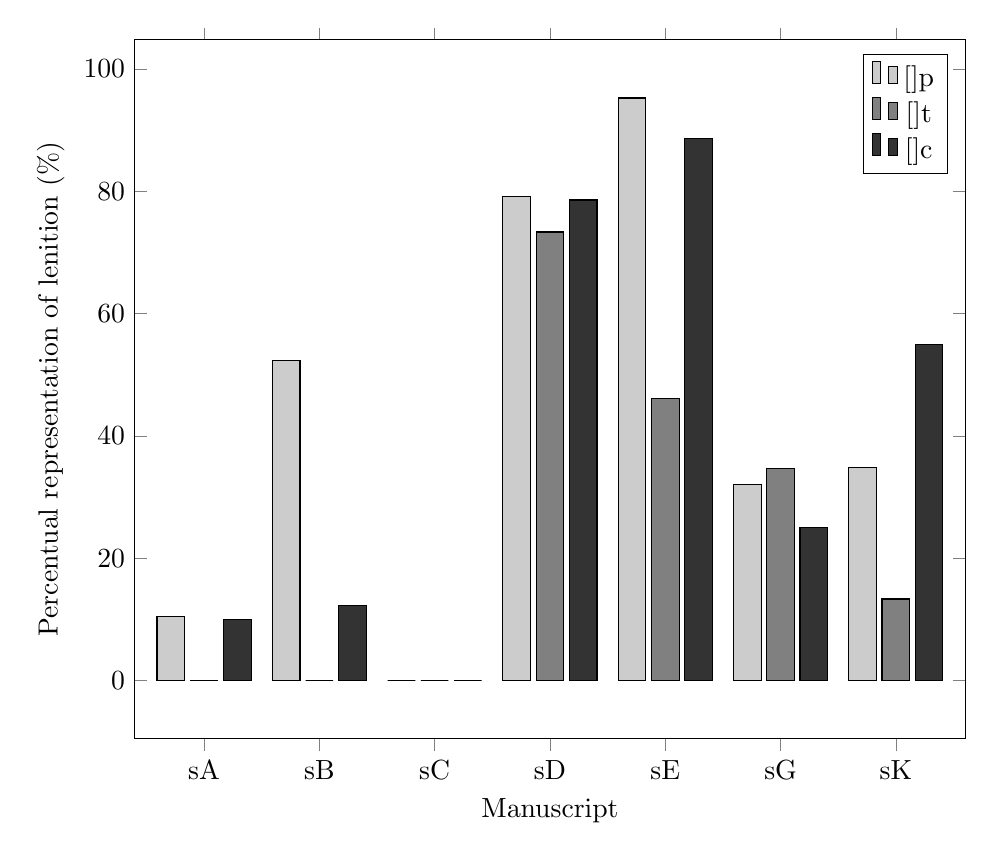
\begin{tikzpicture}
      \begin{axis}[
        ybar,
        width=\textwidth,
        xlabel=Manuscript,
        ylabel={Percentual representation of lenition (\%)},
        symbolic x coords={\gls{sA},\gls{sB},\gls{sC},\gls{sD},\gls{sE},\gls{sG},\gls{sK}},
        xtick=data,
        ]
        \addplot [fill=black!20] coordinates {
          (\gls{sA},10.53)
          (\gls{sB},52.38)
          (\gls{sC},0.00)
          (\gls{sD},79.17)
          (\gls{sE},95.24)
          (\gls{sG},32.00)
          (\gls{sK},34.78)
        };
        \addplot [fill=black!50] coordinates{     
          (\gls{sA},0.00)
          (\gls{sB},0.00)
          (\gls{sC},0.00)
          (\gls{sD},73.33)
          (\gls{sE},46.15)
          (\gls{sG},34.62)
          (\gls{sK},13.33)
        };
        \addplot [fill=black!80] coordinates{
          (\gls{sA},10.00)
          (\gls{sB},12.20)
          (\gls{sC},0.00)
          (\gls{sD},78.57)
          (\gls{sE},88.57)
          (\gls{sG},25.00)
          (\gls{sK},55.00)
        };
        \legend{\mw[]{p},\mw[]{t},\mw[]{c}}
      \end{axis}
    \end{tikzpicture}
    \caption{Percentual representation of lenition of voiceless stops in the various recensions of the tractate on suretyship, excluding research exceptions.}
    \label{fig:barchartlaws}
  \end{figure}

\section{Chronology and the laws}
\label{sec:chronology-laws}


How well do these percentages correspond to the date of composition of the manuscript? The hypothesis is that a law manuscript's orthography will be more conservative than that of a contemporary manuscript containing the \mw{Brut}, because the former would be a copy of an older Welsh-language exemplar, and the latter would be a roughly contemporaneous translation.

\subsection{The apparent age of \gls{sA} \& \gls{sC}}
\label{sec:glsa--glsc}


Purely based on whether lenition of voiceless stops was written. \gls{sA} and \gls{sC} stand out as the most archaic. Neither of these manuscripts writes lenition of \mw{p, t c} aside from a handful of instances. This handful of instances is always found in \gls{sA}, and is presented in Table~\ref{tab:lenptcsa}.

Orthographic lenition of \mw[whose \ldots\ is]{bieu} may be indicative that this verb was petrified here. Lenition here would be due to verbal particle \mw[]{a}, but this particle is not in fact expressed. Also, \mw[]{bieu} is an irregular inflection. Most irregular inflections are forms with \mw[to be]{bod}, so there is grounds for \mw[whose \ldots\ is]{[a]\gls{l} bieu} to be reanalysed as starting with a radical \mw[]{b} rather than a lenited \mw[]{p}.

\begin{table}[h]
  \centering
    \begin{tabular}{ddwql}
    \toprule
    \tch{Page} & \tch{Line} & \tch{Word} & \tch{Translation} & \tch{Reason} \\
    \midrule
    43 & 26 & bieu & owns & [\mw{a}] \\
    45 & 27 & bieu & owns & [\mw{a}]  \\
    46 & 37 & gredu & believe & \mw{e} ‘his' \\
    47 & 22 & genedel & family & \mw{o}  \\
    47 & 24 & g/enedel & family & \mw{o}  \\
    \bottomrule
    \end{tabular}%
\caption{Instances of orthographical lenition of voiceless stops in \gls{sA}.}
  \label{tab:lenptcsa}
\end{table}

\subsection{The apparent age of \gls{sB}}
\label{sec:apparent-age-glssb}


The next most archaic-looking orthography of lenited voiceless stops is found in \gls{sB}, where \mw{t} is never lenited, and \mw{p} and \mw{c} are lenited sporadically. This distribution is puzzling, as it conforms to no pattern found in Chapter~\ref{cha:indep-comp-mwbr}\todo{\& also Taliesin}. There, we witnessed an intermediate period in the development of orthographical lenition of \mw{p, t, c} where \mw{p, t} were not lenited, but where \mw{c} was. Table~\ref{tab:lenpsbexre} shows that there is no obvious pattern, and a word such as \mw[thing]{peth} is found both lenited and unlenited in the same grammatical contexts.

\begin{table}[h]
  \centering
  \begin{tabular}{ddwql}
    \toprule
    \tch{Folio} & \tch{Line} & \tch{Word} & \tch{Translation} & \tch{Reason} \\
    \midrule
    20r & 23 & beth & thing & \mw{ar} \\
    20r & 26 & pleyt & party & \mw{due} \\
    20r & 26 & byeu & owns & [\mw{a}] \\
    20r & 27 & pleyt & party & \mw{due} \\
    20v & 26 & parth & part & \mw{o} \\
    21r & 24 & pleyt & party & \mw{due} \\
    21r & 26 & beth & thing & \mw{ar} \\
    21r & 29 & beth & thing & \mw{ar} \\
    21r & 29 & beth & thing & \mw{ar} \\
    21v & 1 & beth & thing & \mw{ar} \\
    21v & 10 & peth & thing & \mw{ar} \\
    22r & 16 & beth & thing & \mw{am} \\
    22v & 17 & pen & above & prep.\ adj. \\
    23r & 2 & beth & thing & \mw{ar} \\
    23r & 16 & brynno & may buy & \mw{pan} \\
    23r & 18 & perchen & own & \mw{gan} \\
    23r & 23 & peth & thing & \mw{ar} \\
    23r & 25 & perchennauc & owner & \mw{o} \\
    23r & 29 & beth & thing & prep.\ adj. \\
    23v & 1 & beth & thing & prep.\ adj. \\
    23v & 15 & peth & thing & \mw{ar} \\
    \bottomrule
  \end{tabular}%
  \caption{Lenition of \mw{p} in \gls{sB}, excluding research exceptions.}
  \label{tab:lenpsbexre}%
\end{table}%


So what historical context could have induced the scribe of \gls{sB} to add orthographical lenition of \mw{p}, but only in half the cases, and not for \mw{c, t}? \Gls{sB} dates from the second half of the thirteenth century. This is exactly the period when orthographical lenition of \mw{c} became commonplace, but not yet \mw{p, t}.\todo{Unsolved issue}

\subsection{The apparent age of \gls{sG}}
\label{sec:apparent-age-glssg}

The next most ancient-looking orthography of lenited voiceless stops is found in \gls{sG}. Different voiceless stops are all represented to a similar degree, but only about a quarter to a third of lenited \mw{p, t, c} are represented as such. This begs the question whether there is any way to account for the distribution of represented and unrepresented lenition. Some regularities may be found. Scribal abbreviations such as the one given in Example~\ref{abbrsg} never show lenition, perhaps because writing lenition here would make abbreviation unrecognizable.
\mwcc[abbrsg]{\gls{sG} 22v.11}{O d\abbr{eruyd}. y wreic rodi bri duỽ ar peth a'e wadu yn \al{k\abbr{yfreith}aỽl}}{If a woman happens to give an oath and to deny it lawfully}
Also, most instances of \mw[his]{y} are followed by orthographical lenition, perhaps in order to disambiguate this pronoun from the article.

Otherwise, lenition is quite haphazardly represented, and the same grammatical context may show orthographical lenition in one instance, but not in the next. No frequently-occurring grammatical context always has lenition, or never has it. This is significant in itself, because it demonstrates that the scribe of \gls{sG} had the ability to insert lenition, but that it had a low priority for him. He would never do so where it could render an abbreviation unintelligible, and he would do so more frequently only where lenition could serve to make meanings clearer.

\subsection{The apparent age of \gls{sE}}
\label{sec:apparent-age-glsse}

In \gls{sE}, lenition of \gls{T} is written more frequently than in \gls{sG}, even though \gls{sE} is dated from the latter half of the thirteenth century while \gls{sG} is dated from the beginning of the fourteenth century. The orthography of lenition therefore makes this manuscript look younger. Still, a clue exists as to \gls{sE}'s earlier date: lenition of \mw{c} is written  more frequently than that of \mw{t}. It is typical of late thirteenth-century orthography to write lenition of \mw{c}, but not \mw{p} and \mw{t}. \todo{what about \mw{p}?}

\subsection{The apparent age of \gls{sD}}
\label{sec:apparent-age-glssd}

Lenition in \gls{sD} looks the youngest, and indeed the manuscript dates from as late as the early fifteenth century. The reason \gls{sD} looks so much younger than the other manuscripts is not only that it writes lenition with a fairly high frequency, but also that this frequency is similar for \mw{p}, \mw{t}, and \mw{c}. If the total percentage of representation of \lT\ were similar, but much higher for \mw{c} than for \mw{p, t}, then this would have implied an earlier date for \gls{sD}. Remaining instances of non-represented lenition include scribal abbreviations similar to the one found in  Example~\ref{abbrsg}, and instances where  \mw[would be]{bei} may be considered either a verb or a conjunction. Lenition following an elided verbal particle \mw{a} would be expected in the former case, but not in the latter. An instance of this is given in Example~\ref{peisd}.
\mwcc[peisd]{\gls{sD} 29.16--17}{ef a dyly y gymheỻ ual y kymheỻei y mach \al{pei} byỽ.}{He is entitled to compel him as he would compel the surety if he were alive.}

\subsection{The apparent age of \gls{sK}}
\label{sec:apparent-age-glssk}

\gls{sK} looks innovative and conservative at the same time. It tends not to add lenition to voiceless stops wherever lenition was obviously spoken in the earlier period \eg after \mw[on]{ar}. At the same time, however, the scribe of \gls{sK} changed many sentences by removing the element causing lenition, or by adding a word between the element causing lenition and the word to be lenited otherwise.

  It also adds many innovative instances of lenition, \ie object lenition, lenition of the nominal predicate and parenthesis. The implication is that the grammar of the scribe was indeed as new as the fifteenth century, but that his exemplar was very archaic indeed. Perhaps more so than D.

  Another reason besides simply comparing lenition of voiceless stops as a whole makes one think \gls{sK}'s exemplar was more archaic than D's exemplar: orthographical lenition is more frequently expressed for \mw[]{c} than for \mw[]{p} and \mw[]{t}. Because this pattern is otherwise only found in manuscripts from the late thirteenth and early fourteenth century, it implies that \gls{sK} had an intermediate exemplar from this period.

\section{Stemmatics and the laws}
\label{sec:stemmatics-laws}


How well do these percentages showing the prevalence of orthographical lenition mirror the stemmatic relationship between the manuscripts proposed in Figure~\ref{fig:suretyshstemma2} and Figure~\ref{fig:stemmalawc}? Both stemmata propose a close relationship between \gls{sA} and \gls{sE}, and another grouping of \gls{sB}, \gls{sD}, and \gls{sG}. Is the grouping of \gls{sA}\gls{sE} and \gls{sB}\gls{sD}\gls{sG}\ visible in the patterns of lenition? Can any specific additions of orthographical lenition be connected to hypothetical nodes on either stemma?

The differences between these two stemmata concern the position of \gls{sC}, and whether \gls{sG} has a closer relationship with \gls{sB}, or with \gls{sD}. How closely does lenition in \gls{sC} pattern with \gls{sB}\gls{sD}\gls{sG} on the one hand, and with \gls{sA}\gls{sE} on the other hand?  

\begin{figure}[h]
  \newlength{\stemmalen}
  \setlength{\stemmalen}{2.5cm}
  \centering
  \begin{forest} for tree={font=\itshape,l=10mm,l sep=0mm,s sep=3mm,delay={where content={}{shape=coordinate}{}}}
    [X
    [α
    [γ
    [Α,l=20mm]
    [Ε,l=25mm]
    ]
    [C,l=30mm]
    ]
    [β
    [δ
    [D,l=5.3cm,s=-6mm]]
    [ε
    [G,l=35mm,s=-6mm]
    [ζ,s=6mm
    [B,l=15mm]
    [K,l=5.5cm,s=6mm]
    ]
    ]
    ]
    ]
    \node at (forest cs:l=3cm,s=\stemmalen +.5cm) {1200};
    \node at (forest cs:l=5cm,s=\stemmalen +.5cm) {1300};
    \node at (forest cs:l=7cm,s=\stemmalen +.5cm) {1400};
    \node at (forest cs:l=9cm,s=\stemmalen +.5cm) {1500};
    \draw[dotted] (forest cs:l=3cm, s=-\stemmalen) -- (forest cs:l=3cm, s=\stemmalen);
    \draw[dotted] (forest cs:l=5cm, s=-\stemmalen) -- (forest cs:l=5cm, s=\stemmalen);
    \draw[dotted] (forest cs:l=7cm, s=-\stemmalen) -- (forest cs:l=7cm, s=\stemmalen);  
    \draw[dotted] (forest cs:l=9cm, s=-\stemmalen) -- (forest cs:l=9cm, s=\stemmalen);  
  \end{forest}
  \begin{forest} for tree={font=\itshape,l=10mm,l sep=0mm,s sep=3mm,delay={where content={}{shape=coordinate}{}}}
    [\textup{Redaction I}
    [α
    [Α,l=30mm]
    [Ε,l=35mm]
    ]
    [\textup{Redaction II}
    [β
    [C,l=20mm]
    ]
    [γ,
    [
    [D,s=-6mm,l=4.3cm]
    [G,l=25mm]]
    [
    [B,s=6mm,l=15mm]
    [K,l=55mm]
    ]
    ]
    ]
    ]
    ]
    \node at (forest cs:l=3cm,s=\stemmalen +.5cm) {1200};
    \node at (forest cs:l=5cm,s=\stemmalen +.5cm) {1300};
    \node at (forest cs:l=7cm,s=\stemmalen +.5cm) {1400};
    \node at (forest cs:l=9cm,s=\stemmalen +.5cm) {1500};
    \draw[dotted] (forest cs:l=3cm, s=-\stemmalen) -- (forest cs:l=3cm, s=\stemmalen);
    \draw[dotted] (forest cs:l=5cm, s=-\stemmalen) -- (forest cs:l=5cm, s=\stemmalen);
    \draw[dotted] (forest cs:l=7cm, s=-\stemmalen) -- (forest cs:l=7cm, s=\stemmalen);  
    \draw[dotted] (forest cs:l=9cm, s=-\stemmalen) -- (forest cs:l=9cm, s=\stemmalen);  
  \end{forest}
  \caption{Two stemmata}
  \label{fig:twostemmata}
\end{figure}

\subsection{The two groups}
\label{sec:two-groups}
Here, I discuss how the orthography of lenition may aid in deciding on the position of \gls{sC} within a stemma of manuscripts, and whether \gls{sG} has a more direct stemmatic relationship with \gls{sB}, or with \gls{sD}.

The discussion of these points allows me to introduce several methodological tools.
\subsubsection{Hypercorrection}
\label{sec:hypercorrection}


One thing \gls{sA} and \gls{sE} uniquely have in common is that they both contain one instance of unlenited \mw{ll} where we would expect lenition. These instances are given in Examples~\ref{ex:sigallw} and \ref{ex:sigellw}.
\begin{mwl}
  \mwc[ex:sigallw]{\gls{sA} 45.14--15}{a heny vrh \al{ll}u e macht.\ kanis macht adeuedic yu.}{and that on the oath of surety, since he is an acknowledged surety.}
  \mwc[ex:sigellw]{\gls{sE} 35.32--33}{a hynny urth \al{ll}v y mach canys mach adeuedyc yu
  }{and that on the oath of surety, since he is an acknowledged surety.}
\end{mwl}


The consonant \mw{ll} is unique among all \gls{mw} consonants in that its lenited form is more archaic than its radical form in the orthography. This means that lack of orthographical lenition of \mw[]{l}--- usually a sign of archaism --- is in fact a shared innovation between \gls{sA} and \gls{sE}. I consider this type of hypercorrection a low-probability event, so it is  near-impossible that this was done separately in each manuscript.  This suggests that these two manuscripts share a common ancestor not shared by any other manuscripts studied here.

Unlike \gls{sA}\gls{sE}, \gls{sC} has a lenited consonant here, as shown in \ref{ex:sigcllw}.
\mwcc[ex:sigcllw]{\gls{sC} 157rb.14--16}{a henny wrth \al{l}w e mach. kanys mach adeỽedyc ew.}{and that on the oath of surety, since he is an acknowledged surety}
Because \gls{sC} does not pattern with \gls{sA}\gls{sE}, there is no evidence that \gls{sC} forms a group with these two manuscripts. However, it is not  evidence for grouping with the other manuscripts either, because the reading \mw{wrth lw}  found in \gls{sC} and all the other manuscripts is a shared archaism\footnote{One might argue that there is little phonetic difference between \mw[]{-th l-} and \mw[]{-th ll-}. Even if this plays a role in writing lenition of \mw[]{ll}, there would be little reason to innovate towards \mw[]{ll}, precisely because there is no difference.}. 

No other instances of hypercorrection exist that are shared between more than one mansucript.

Another instance of hypercorrection, with interpretation of a third person plural possessive pronoun as a third person singular, and subsequent lenition, and also with an instance of failing to lenite \mw{p} because \mw[on]{ar} was taken to be \mw[and]{ac}:
\mwcc[]{\gls{sK} 71.22--23}{O d\abbr{eruyd} i dyn rodi llaỽer o ueichieu a peth a mynnu i ỽadu oꝛ kynogyn.}{If a man happens to take many sureties on a thing and wishes to deny them from the debtor.}

Hypercorrection of adding lenited \mw[]{g}:
\begin{mwl}
\mwc[]{\gls{sK} 77.13--14}{Ac na dyly hitheu raith o ỽyr i \al{ỽadu} git a hi}{here \mw[her]{i} causes lenition as it meant `him'.}
\mwc[]{\gls{sD} 61.6}{ac nadyly hitheu reith o wyr y gỽadu hi.}{}
\end{mwl}
\subsubsection{Object lenition}
\label{sec:object-lenition}

Object lenition is a type of free lenition not applied consistently in Middle Welsh, especially not in its earlier stages. Unlike the matter of the voiceless stops, lenition or non-lenition of the grammatical object is not simply a matter of orthography, but rather reflects spoken free variation.

Consider object lenition of \mw[that \dots\ is]{bot} in Examples~\ref{ex:sbbot}, \ref{ex:scbot}, and \ref{ex:sdbot} below:

\begin{mwl}
  \mwc[ex:sbbot]{\gls{sB} 21r.14--16}{ac os negyd uyd e kennogen ydau deuet ar e uach a holet e uach a dywedet \al{bot} e kynnogen en negyd ydau. }{And if the debtor will be a refuser to him, he must come to the surety and must claim to the surety and must say that the debtor is a refuser.}
  \mwc[ex:scbot]{\gls{sC} 156vb.18--23}{ac os negyf ỽyd e kynnogyn ydaw; deỽet ar y ỽach a holet y ỽach. a dywedet \al{ỽot} e kynnogyn en negyf ydaỽ.}{And if the debtor will be a refuser to him, he must come to the surety and must claim to the surety and must say that the debtor is a refuser.}
  \mwc[ex:sdbot]{\gls{sD} 54.26--55.3}{ac os negyf vyd y kynnogyn idaỽ; deuet ar y vach a holet y uach. a dywedet \al{vot} y kynnogyn yn negyf idaỽ.}{And if the debtor will be a refuser to him, he must come to the surety and must claim to the surety and must say that the debtor is a refuser.}
  \mwc[]{\gls{sK} 71.4--6}{ac os negyd uyd y kynnogyn ido. deuet ar i uach a dyỽetet \al{uot} y kynnogyn yn negyd ido.}{}

\end{mwl}

Manuscript \gls{sC} patterns with \gls{sD} in this regard. This is a shared innovation that does not necessarily occur everywhere, so lenition of \mw[]{bot} is diagnostic of \gls{sC} and \gls{sD} sharing a stemmatic node not shared with \gls{sB}. This innovation could occur independently, so using object lenition to demonstrate shared innovations is best served by having several examples at hand.

\begin{mwl}
  \mwc[]{\gls{sK} 77.7--9}{ac ỽꝛth naill y mach \al{gynnal} ẏ uechni ir aeth yn uach arnei i gelỽir un oueruach}{}
  \mwc[]{\gls{sD} 60.25--26}{ac ỽrth na eiỻ y mach \al{kynnal} y vechni yd aeth yn vach arnei y gelwir yn oueruach.}{}
\end{mwl}

\subsubsection{NP lenition}
\label{sec:np-lenition}

\begin{mwl}
  \mwc[]{\gls{sA} 47.19}{kan  bu guell kanthau ef uunet...}{}
  \mwc[]{\gls{sB} 23r.7--8}{a  chan bu well ganthau ef menet}{}
  \mwc[]{\gls{sC} 160ra.10--12}{kan bw gwell kanthaw ef mynet...}{}
  \mwc[]{\gls{sD} 59.24--25}{kann bu weỻ ganthaỽ vynet...}{}
  \mwc[]{\gls{sE} 38.14}{kanbu well ganthaỽ ew mynet }{}
  \mwc[]{\gls{sK} 76.6--7 \S 64.12}{kan bu ỽell gando mynet...}{}
\end{mwl}

\subsubsection{Adverb lenition}
\label{sec:adverb-lenition}

\begin{mwl}
  \mwc[]{\gls{sK} 73.1--2}{Ni dyỽeit y .k\abbr{yfreith}.\ dylyu ohonaỽ trachefyn namyn dimai}{}
  \mwc[]{D 56.19--20}{Ny dyweit.\ kyfreith.\ dylyu ohonaỽ drachefyn namyn dimei.}{}
\end{mwl}
This makes \gls{sK} orthographically more conservative than the percentages suggest.

\subsubsection{variable gender}
\label{sec:variable-gender}

\mwcc[]{\gls{sK} 70.11-12}{yn gyneſſet ac u dlyỽynt talu galanas git ac ef ai \al{gymryt}}{as close as if they would have to pay wergild with him or to take it.}

The word \mw[wergild]{galanas} is masculine in \gls{sK}, but feminine in \gls{sD}.

\subsubsection{Renewing or old vocab}
\label{sec:renewing-or-old}

\mwcc[]{K 70.21--22, \S 60.6}{kani oꝛuc e hun teithi mach}{For he himself did not release a suretyship}

Other MSS use \mw[did]{gwnaeth}, which is typically indicative of a later composition.
\subsubsection{Voiceless stops}
\label{sec:voiceless-stops}

Most manuscripts discussed in this chapter date from the thirteenth century. The two exceptions are \gls{sD} and \gls{sG}. A newly composed text in the fourteenth century or later would  have full orthographical lenition of voiceless stops.

Manuscripts \gls{sD} and \gls{sG}, however, have only partial orthographical lenition of voiceless stops. Instances of non-lenition are therefore traces of an orthographically more archaic exemplar.

Wherever lenition of this type occurs in the same place in both \gls{sD} and \gls{sG}, we are dealing with a shared innovation. Shared innovations are diagnostic of a stemmatic relationship.


\begin{mylongtable}{ddwqllw}
\toprule
\tch{Page} & \tch{Line} & \tch{Word} & \tch{Translation} & \tch{Cause} & \tch{Shown} & \tch{C} \\
\midrule
68 & 20 & peth & thing & \mw{ar} & No & p \\
68 & 21 & tri & three & \mw{o} & No & t \\
68 & 22 & talu & pay & \mw{o} & No & t \\
68 & 24 & bieu & whose … is & [\mw{a}] & Yes & p \\
68 & 24 & bla/it & party & \mw{dỽy} & Yes & p \\
69 & 11 & k[yfreith] & law & fem.\ art & No & c \\
69 & 15 & gymryt & take & parenthesis & Yes & c \\
70 & 3  & dyngeiſt & you swore & \mw{a} & Yes & t \\
70 & 8  & parth & side & \mw{o} & No & p \\
70 & 8  & tat & father & \mw{y} ‘his' & No & t \\
70 & 8  & parth & side & \mw{o} & No & p \\
70 & 10 & gyneſſet & as close as & \mw{yn} & Yes & c \\
70 & 12 & gymryt & take & \mw{i} ‘his' & Yes & c \\
70 & 21 & gynogyn & debtor & \mw{i} ‘his' & Yes & c \\
71 & 15 & peth & thing & \mw{ar} & No & p \\
71 & 16 & pleit & party & \mw{dỽy} & No & p \\
71 & 18 & peth & thing & \mw{ar} & No & p \\
71 & 20 & peth & thing & \mw{ar} & No & p \\
71 & 20 & peth & thing & \mw{ar} & No & p \\
71 & 22 & peth & thing & {\mw{a}[\mw{r}]} & No & p \\
72 & 4  & k[yfreith] & law & fem.\ art & No & c \\
72 & 6  & dalu & pay & \mw{o} & Yes & t \\
72 & 7  & talu & pay & \mw{hep} & No & t \\
72 & 7  & k[yfreith] & law & fem.\ art & No & c \\
72 & 8  & k[einiawc] & penny & fem.\ art & No & c \\
72 & 9  & gyntaf & first & fem.\ art & Yes & c \\
72 & 10 & peth & thing & \mw{ar} & No & p \\
72 & 11 & talu & pay & \mw{am} & No & t \\
72 & 13 & bieu & whose is & [\mw{a}] & Yes & p \\
72 & 15 & gyntaf & first & fem.\ noun & Yes & c \\
72 & 17 & gyffroi & move & \mw{i} ‘his' & Yes & c \\
73 & 1  & k[yfreith] & law & fem.\ art & No & c \\
73 & 3  & k[einiawc] & penny & fem.\ art & No & c \\
73 & 3  & k[yfreith] & law & fem.\ art & No & c \\
73 & 9  & k[yfreith] & law & fem.\ art & No & c \\
73 & 12 & gymryt & take & \mw{i} ‘his' & Yes & c \\
73 & 15 & gỽbyl & whole & \mw{yn} & Yes & c \\
73 & 18 & talei & paid & \mw{a} & No & t \\
73 & 19 & gymell & instigate & \mw{i} ‘to' & Yes & c \\
73 & 20 & talỽyf & I may pay & \mw{a} & No & t \\
74 & 5  & colledic & lost & \mw{yn} & No & c \\
74 & 6  & peth & thing & \mw{ar} & No & p \\
74 & 7  & k[yfreith] & law & fem.\ art & No & c \\
74 & 16 & gynogyn & debtor & \mw{o} & Yes & c \\
74 & 18 & gynogyn & debtor & \mw{yn} & Yes & c \\
75 & 4  & gollet & loss & fem.\ art & Yes & c \\
75 & 7  & k[yfreith] & law & fem.\ noun & No & c \\
75 & 14 & tat & father & \mw{i} ‘his' & No & t \\
75 & 15 & tat & father & \mw{i} ‘his' & No & t \\
75 & 16 & k[yfreith] & law & fem.\ art & No & c \\
75 & 20 & k[yfreith] & law & \mw{oes} & No & c \\
75 & 20 & k[yfreith] & law & \mw{oes} & No & c \\
76 & 1  & tat & father & \mw{i} ‘his' & No & t \\
76 & 1  & tat & father & \mw{i} ‘his' & No & t \\
76 & 2  & beth & thing & \mw{ar} & Yes & p \\
76 & 11 & genedyl & family & \mw{o} & Yes & c \\
76 & 12 & genedyl & family & \mw{o} & Yes & c \\
76 & 13 & tat & father & \mw{i} ‘his' & No & t \\
76 & 14 & genedyl & family & \mw{o} & Yes & c \\
76 & 14 & tat & father & \mw{i} ‘his' & No & t \\
76 & 16 & bryno & may buy & \mw{pan} & Yes & p \\
76 & 18 & p[er]chen & own & \mw{gan} & No & p \\
76 & 18 & gyfneỽit & exchange & \mw{i} ‘to' & Yes & c \\
76 & 21 & gymello & may compel & \mw{a} & Yes & c \\
76 & 21 & gyfneỽit & exchange & \mw{i} ‘to' & Yes & c \\
76 & 23 & peth & thing & \mw{ar} & No & p \\
77 & 1  & p[er]chen & owner & \mw{o} & No & p \\
77 & 2  & gych/ỽyn & move & \mw{i} ‘his' & Yes & c \\
77 & 5  & gauas & gained & \mw{a} & Yes & c \\
77 & 6  & beth & thing & \mw{pa} & Yes & p \\
77 & 6  & k[yfreith] & law & fem.\ art & No & c \\
77 & 7  & beth & thing & \mw{pa} & Yes & p \\
77 & 8  & gynnal & maintain & obj. & Yes & c \\
77 & 17 & k[yfreith] & law & fem.\ art & No & c \\
77 & 21 & beth & thing & \mw{ar} & Yes & p \\
77 & 22 & k[yfreith]iol & lawful & \mw{yn} & No & c \\
77 & 22 & k[yfreith] & law & fem.\ art & No & c \\
\bottomrule
\caption{Lenited voiceless stops in \gls{sK}.}
\end{mylongtable}

%%% Local Variables:
%%% mode: latex
%%% coding: utf-8
%%% TeX-master: "../main"
%%% End:
